\documentclass{article}
\usepackage[a4paper, total={7in, 9.5in}]{geometry}
\usepackage{amsmath,amsfonts,amsthm,amssymb,graphicx,float, setspace, bm}
\usepackage[utf8]{inputenc}
\usepackage{float}
\usepackage{titlesec}
\usepackage{setspace}
\usepackage{geometry}
\usepackage[style=numeric]{biblatex}
\usepackage[autostyle=true]{csquotes}
\usepackage{breqn}
\usepackage{subfig}
\usepackage[bottom]{footmisc}
\usepackage{adjustbox}
\usepackage{lipsum}
\usepackage{hyperref}
\usepackage[ruled,vlined]{algorithm2e}
\hypersetup{
    colorlinks=true,
    urlcolor=magenta
}
\usepackage[table,x11names]{xcolor}

\usepackage{xltabular}
\usepackage{multirow}
\usepackage{booktabs}


\renewcommand{\baselinestretch}{1.5} 
\setlength\parindent{0pt}
%----------------------------------------------------------------------------------------
%	START
%----------------------------------------------------------------------------------------

\newcommand{\horrule}[1]{\rule{\linewidth}{#1}}

\title{ \normalfont \normalsize 
\huge CPSC 532W - Homework 5}
\date{}
\author{Xiaoxuan Liang - 48131163}
\def\cond{\; | \;}

\begin{document}

\maketitle
Public GitHub repo: https://github.com/Xiaoxuan1121/CPSC532W/tree/main/a5
\begin{enumerate}
\item Program 1:

\begin{figure}[!ht]
	\centering
	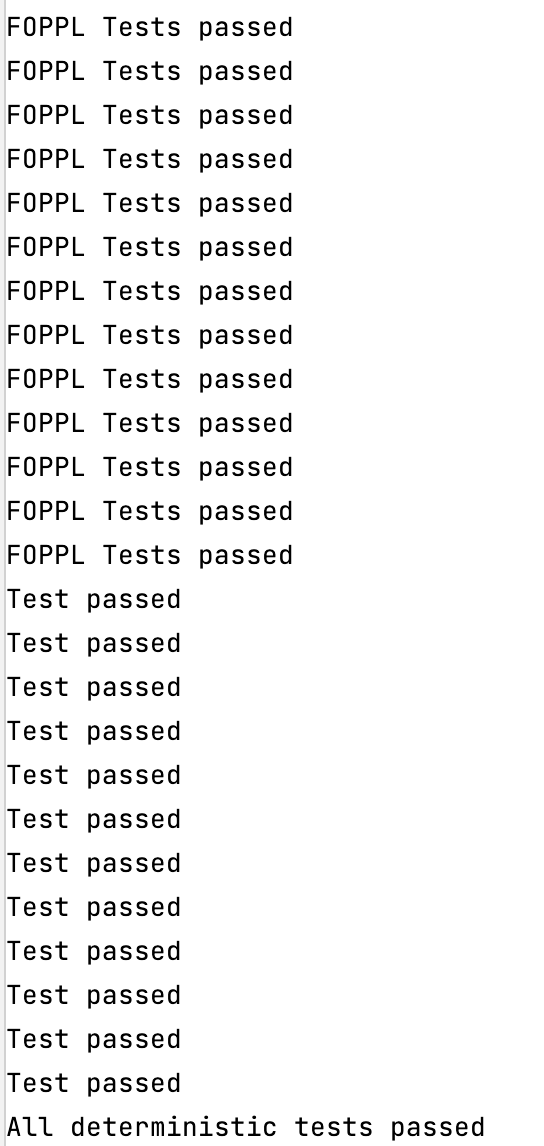
\includegraphics[scale=0.5]{../figs/deterministic_tests}
\end{figure}

\begin{figure}[!ht]
	\centering
	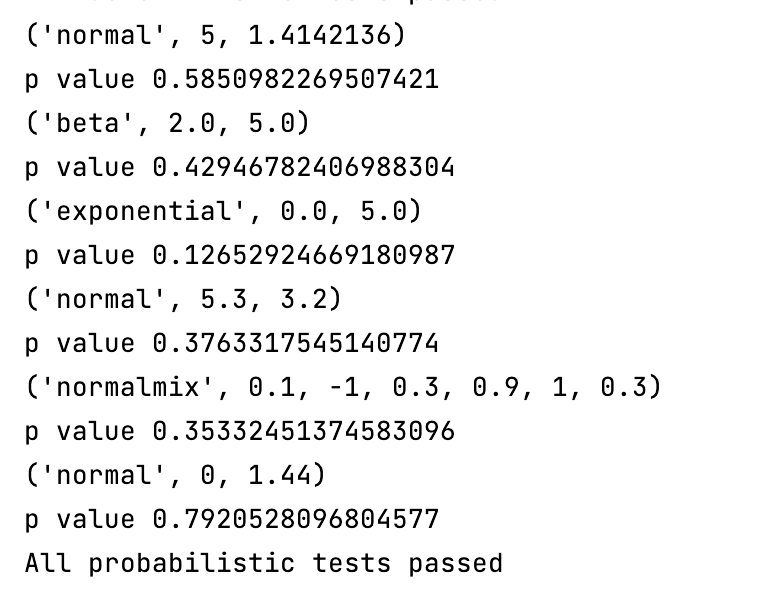
\includegraphics[scale=0.5]{../figs/probabilistic_tests}
\end{figure}

\newpage
\begin{figure}[!ht]
	\centering
	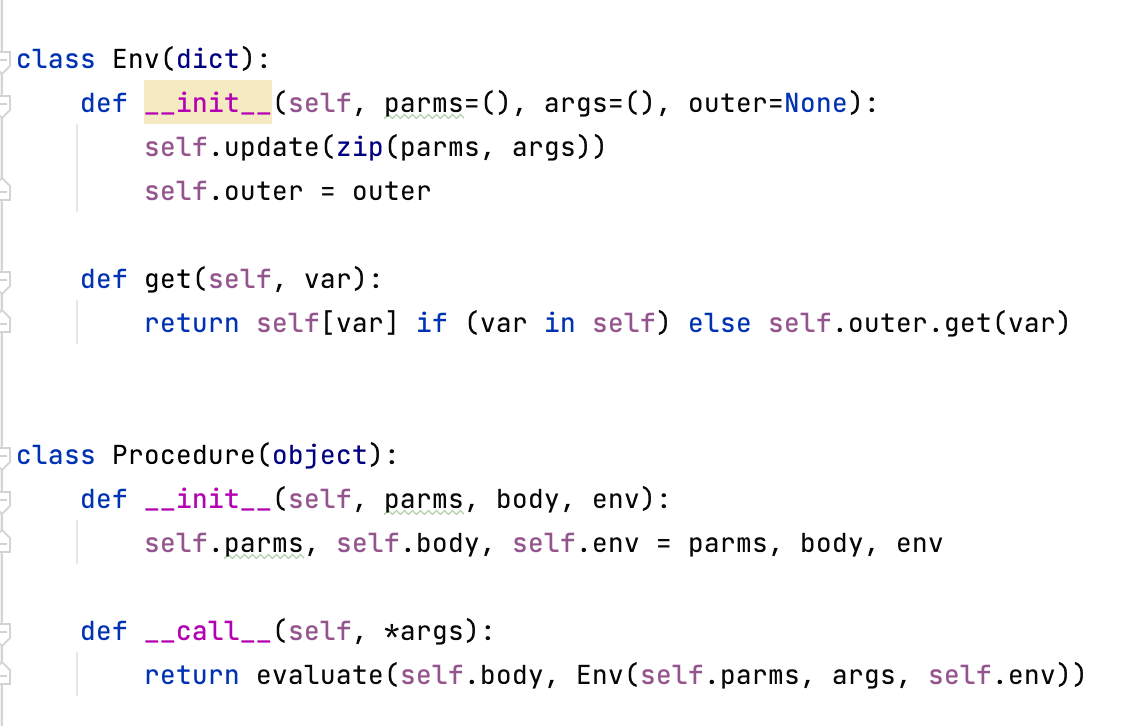
\includegraphics[scale=0.5]{../figs/evaluate_1}
\end{figure}

\begin{figure}[!ht]
	\centering
	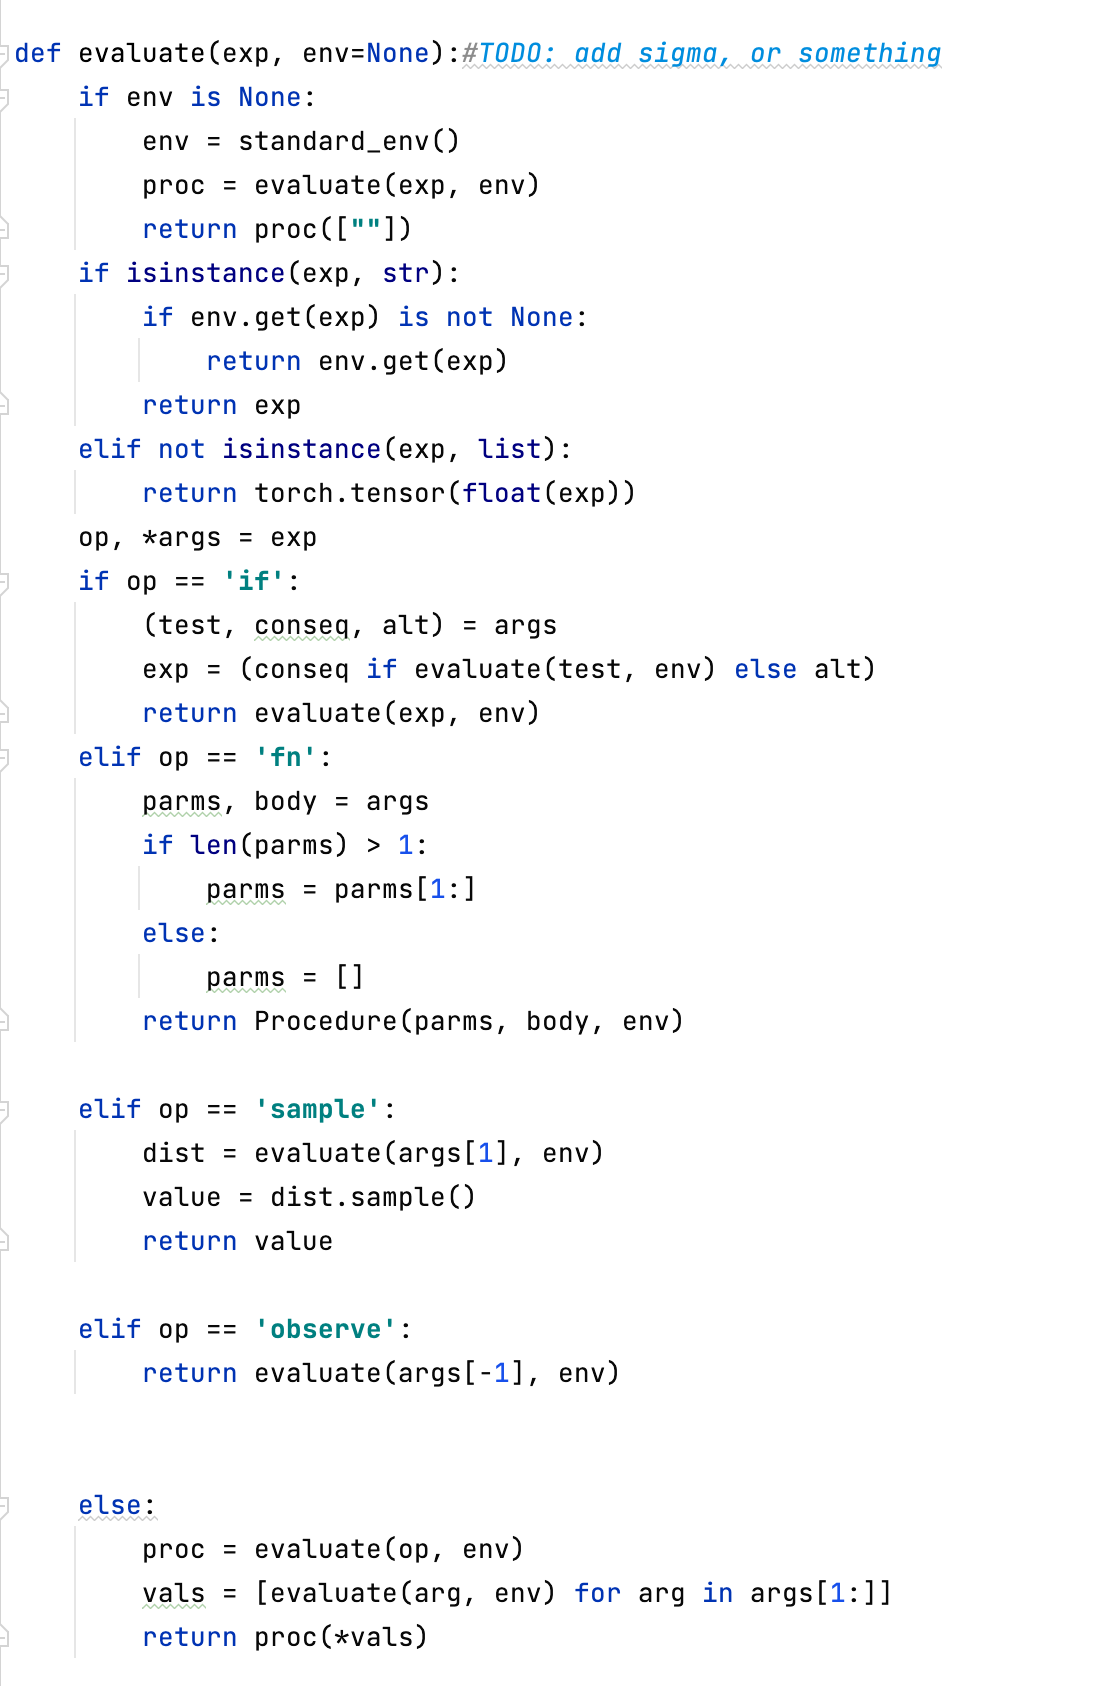
\includegraphics[scale=0.5]{../figs/evaluate_2}
\end{figure}

\newpage
\begin{figure}[!ht]
	\centering
	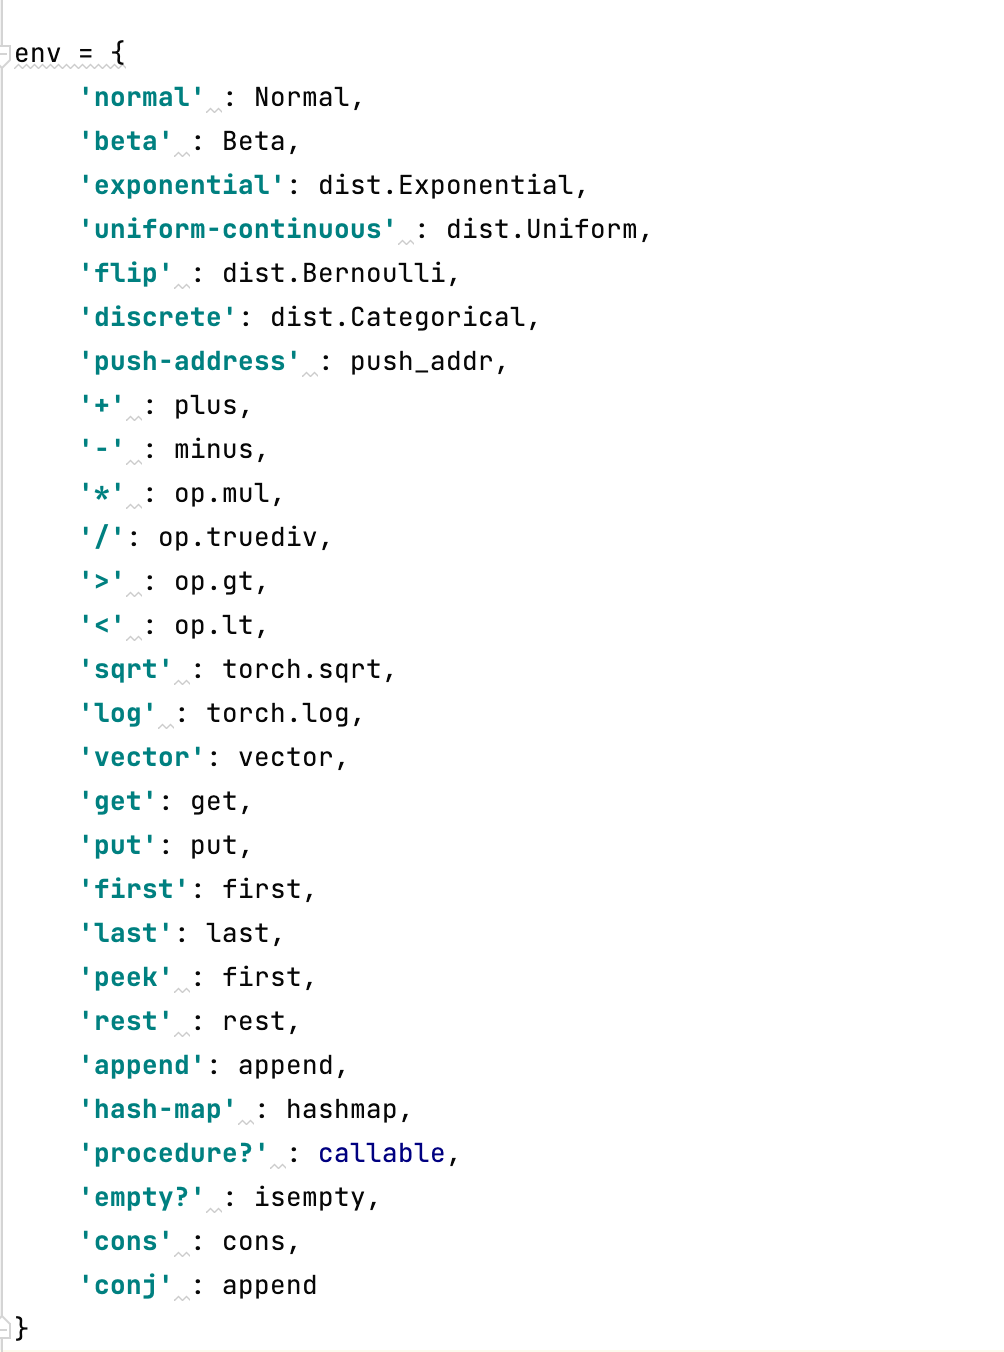
\includegraphics[scale=0.5]{../figs/primitives_1}
\end{figure}

\begin{figure}[!ht] 
	\centering
	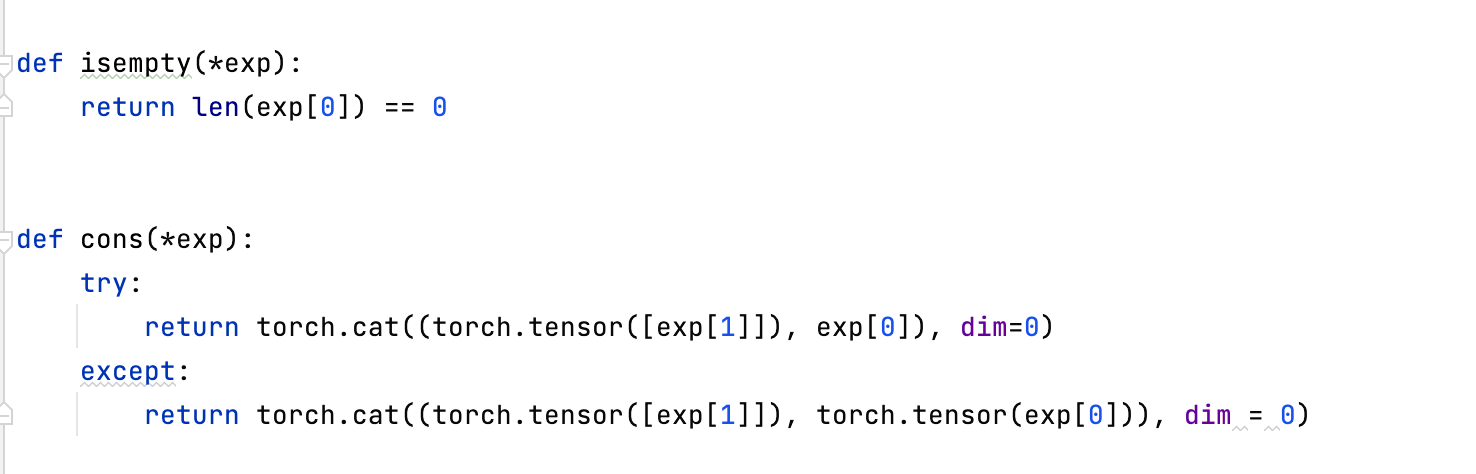
\includegraphics[scale=0.5]{../figs/primitives_2}
\end{figure}

\newpage
\item Program 2:

\begin{figure}[!ht]
	\centering
	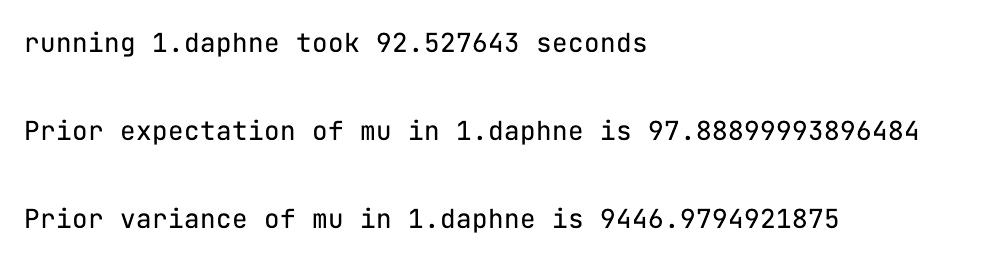
\includegraphics[scale=0.5]{../figs/1_daphne_results}
\end{figure}
\begin{figure}[!ht]
	\centering
	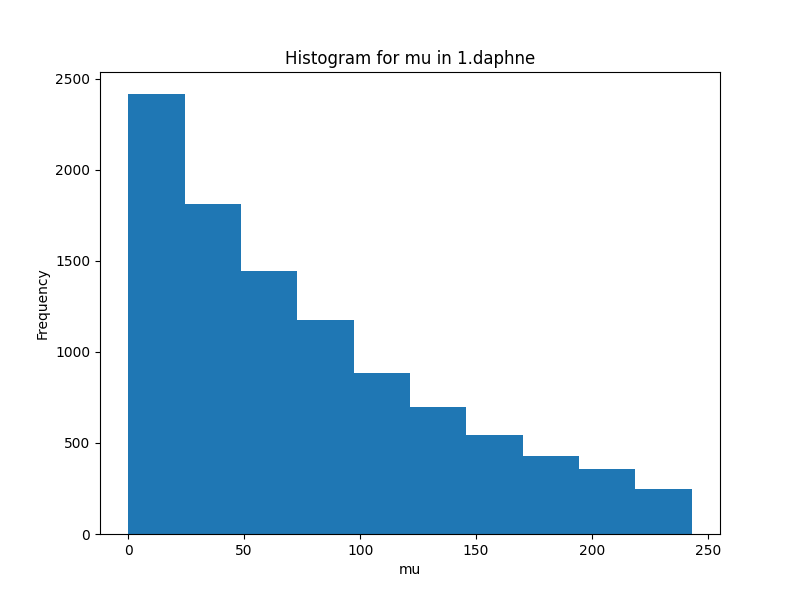
\includegraphics[scale=0.5]{../figs/1_daphne}
\end{figure}

\item Program 3:

\begin{figure}[!ht]
	\centering
	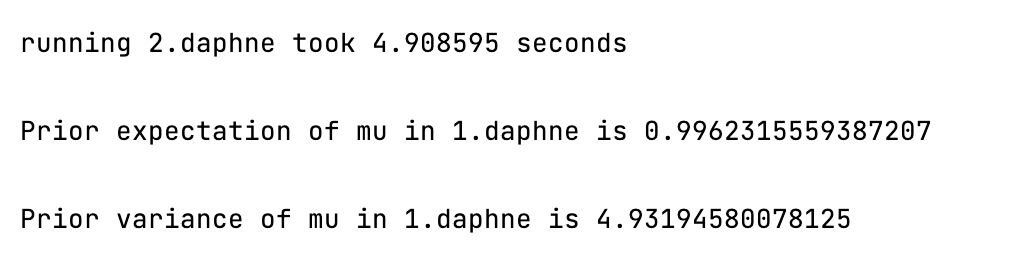
\includegraphics[scale=0.5]{../figs/2_daphne_results}
\end{figure}

\begin{figure}[!ht]
	\centering
	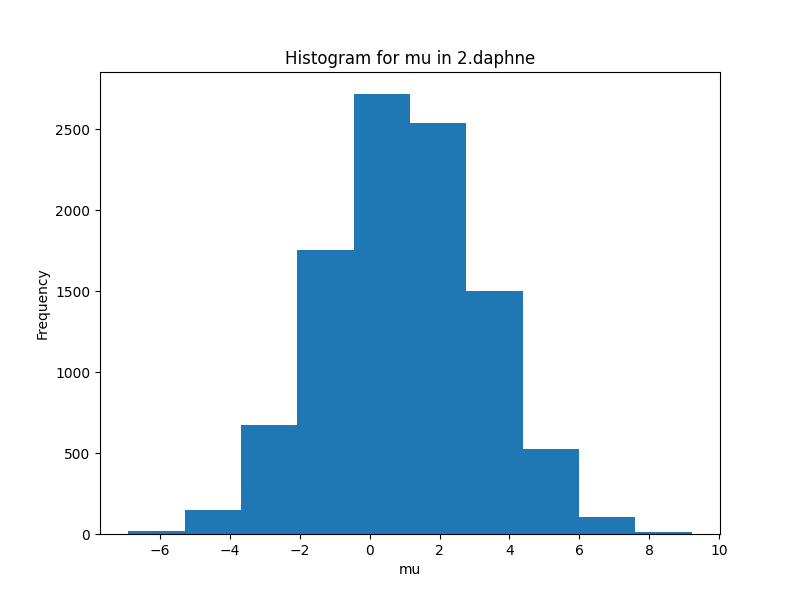
\includegraphics[scale=0.5]{../figs/2_daphne}
\end{figure}

\newpage
\item Program 4:

\begin{figure}[!ht]
	\centering
	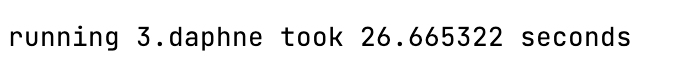
\includegraphics[scale=0.5]{../figs/3_daphne_results}
\end{figure}

\begin{figure}[!htp]
	\centering
	 \subfloat[Samples from the prior for HMM step 1]{%
        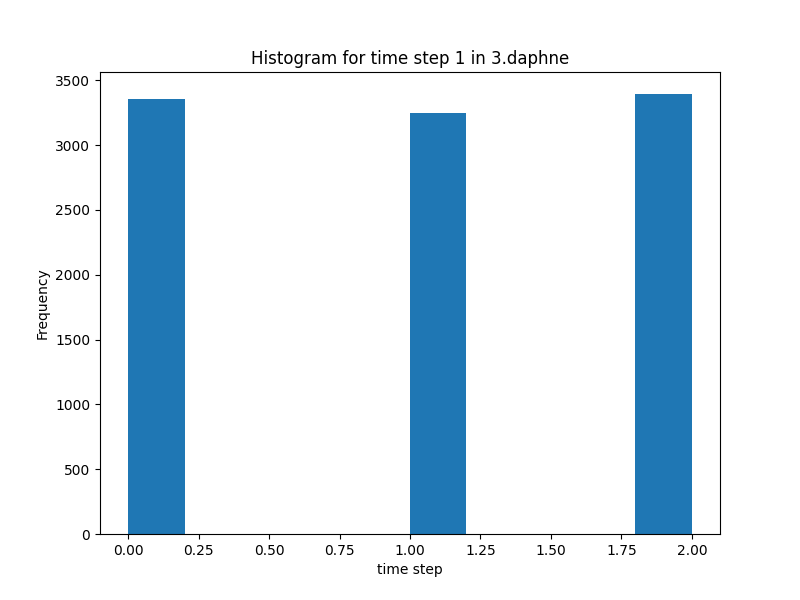
\includegraphics[width=0.2\textwidth]{../figs/4_daphne_1}%
        \label{fig:a}%
        }%
    \hfill%
    \subfloat[Samples from the prior for HMM step 2]{%
        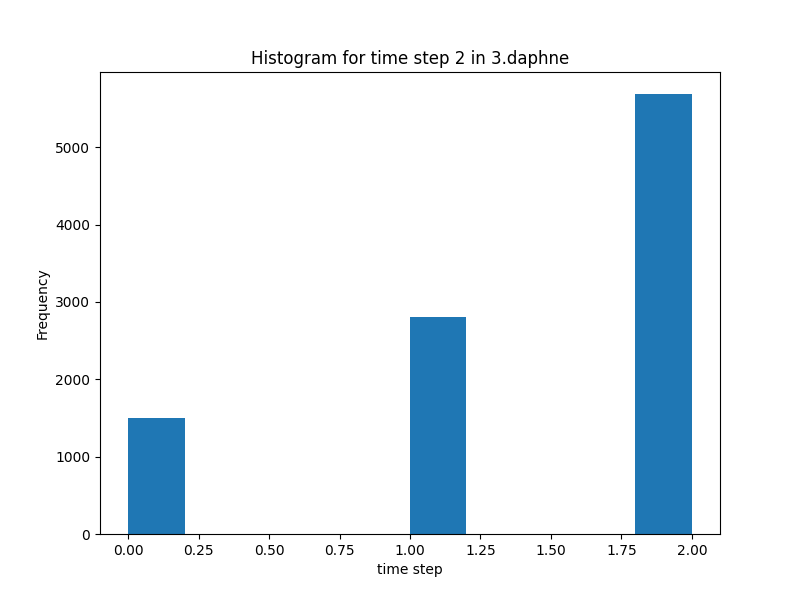
\includegraphics[width=0.2\textwidth]{../figs/4_daphne_2}%
        \label{fig:b}%
        }%
   \hfill%
   \subfloat[Samples from the prior for HMM step 3]{%
   	  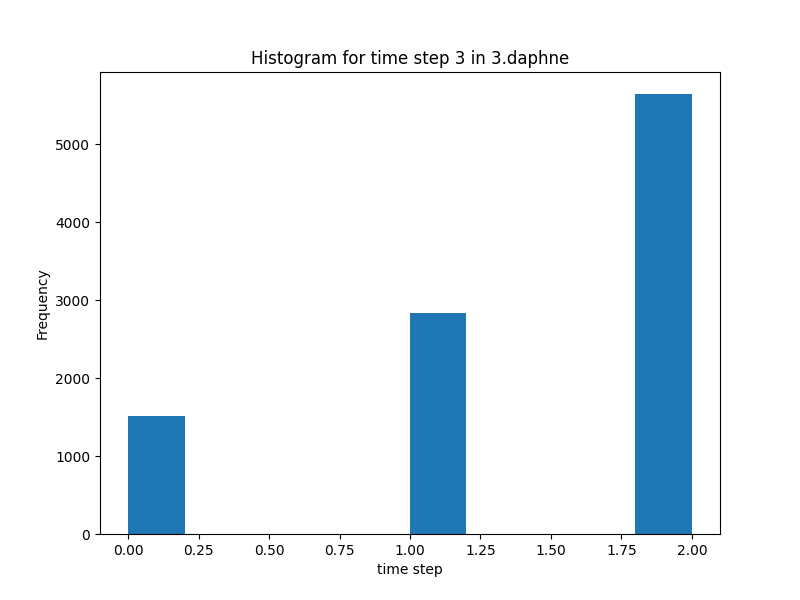
\includegraphics[width=0.2\textwidth]{../figs/4_daphne_3}%
   	  \label{fig:a}%
   	  }%
   \hfill%
	 \subfloat[Samples from the prior for HMM step 4]{%
        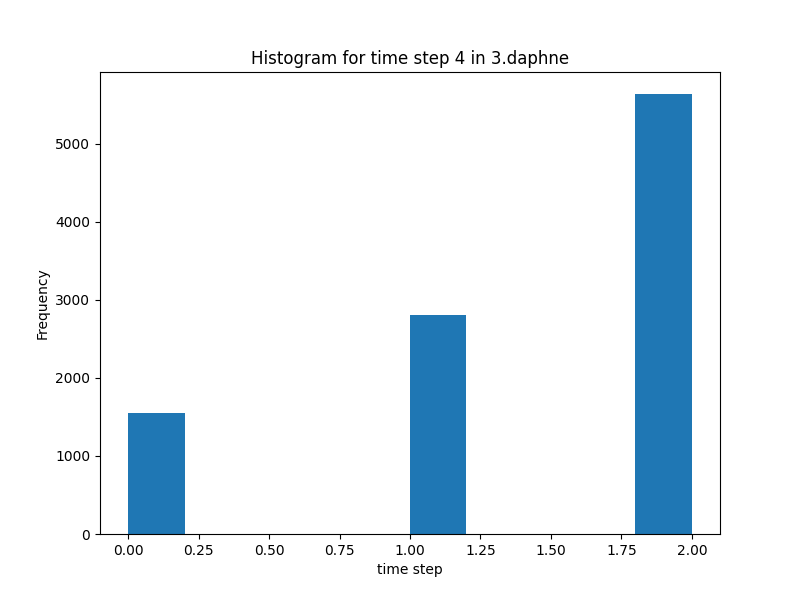
\includegraphics[width=0.2\textwidth]{../figs/4_daphne_4}%
        \label{fig:d}%
        }%
        
   \hfill%
    \subfloat[Samples from the prior for HMM step 5]{%
        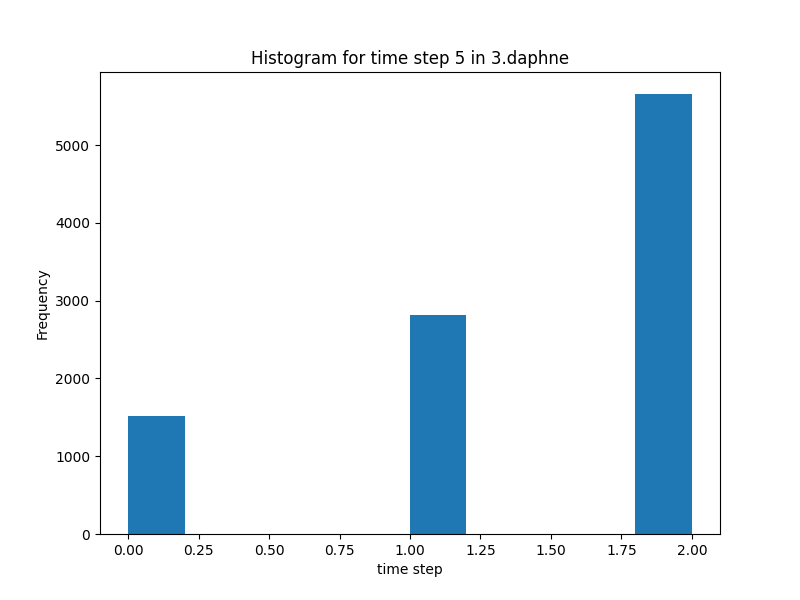
\includegraphics[width=0.24\textwidth]{../figs/4_daphne_5}%
        \label{fig:e}%
        }%
   \centering
   \subfloat[Samples from the prior for HMM step 6]{%
   	  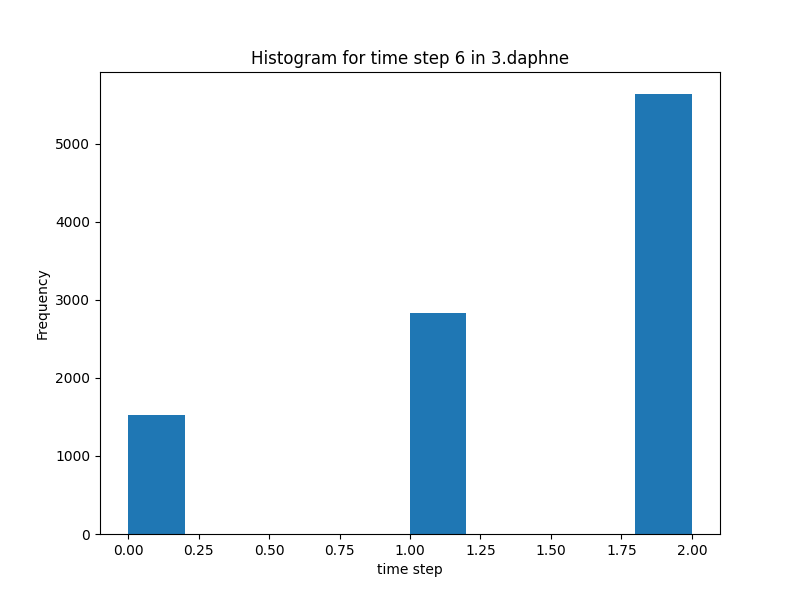
\includegraphics[width=0.24\textwidth]{../figs/4_daphne_6}%
   	  \label{fig:f}%
   	  }%
   \hfill%
	 \subfloat[Samples from the prior for HMM step 7]{%
        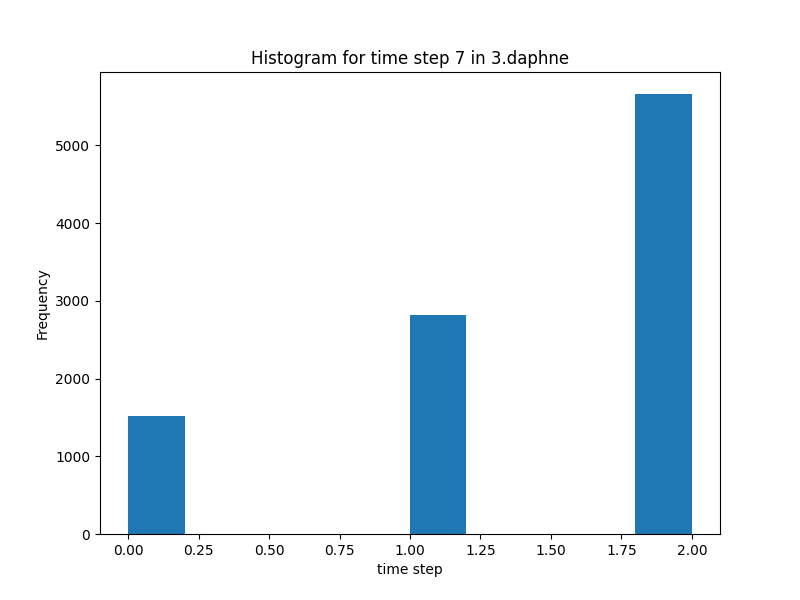
\includegraphics[width=0.24\textwidth]{../figs/4_daphne_7}%
        \label{fig:d}%
        }%
   \hfill%
    \subfloat[Samples from the prior for HMM step 8]{%
        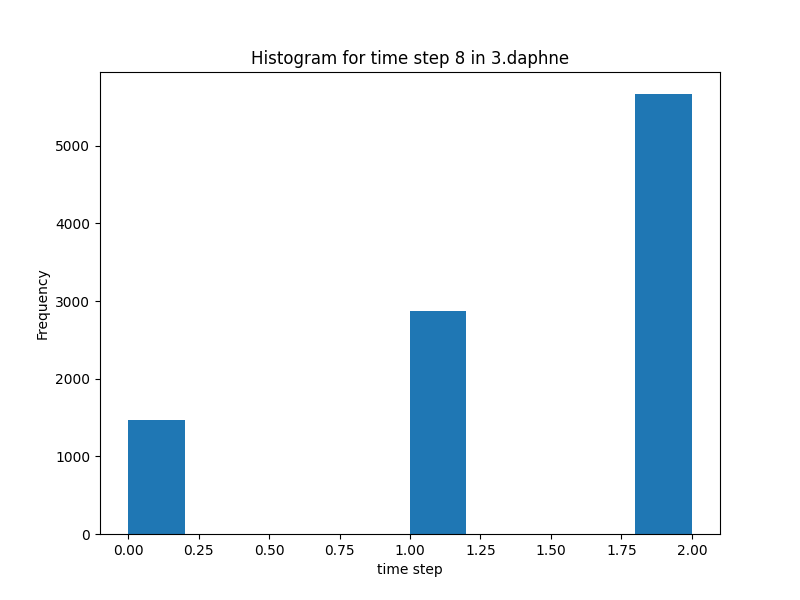
\includegraphics[width=0.24\textwidth]{../figs/4_daphne_8}%
        \label{fig:e}%
        }%
        
   \centering
   \subfloat[Samples from the prior for HMM step 9]{%
   	  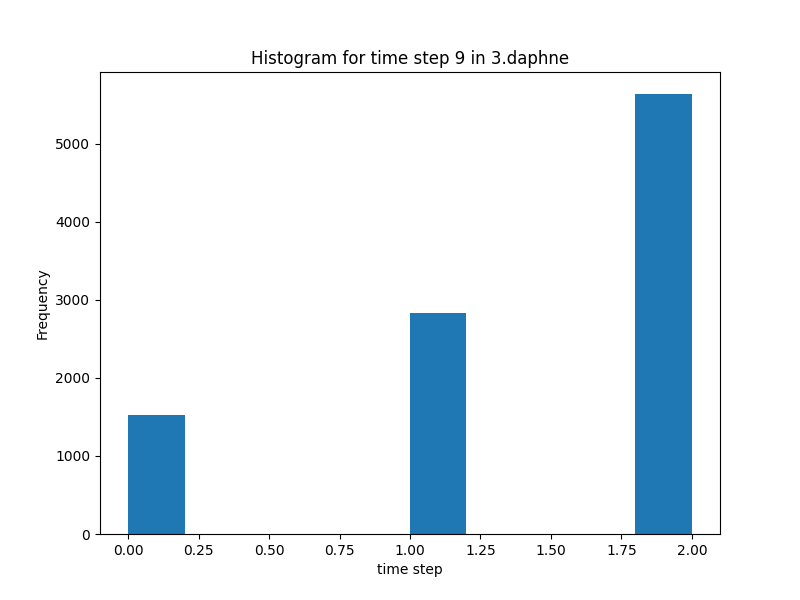
\includegraphics[width=0.24\textwidth]{../figs/4_daphne_9}%
   	  \label{fig:f}%
   	  }%
   \hfill%
   	  \subfloat[Samples from the prior for HMM step 10]{%
        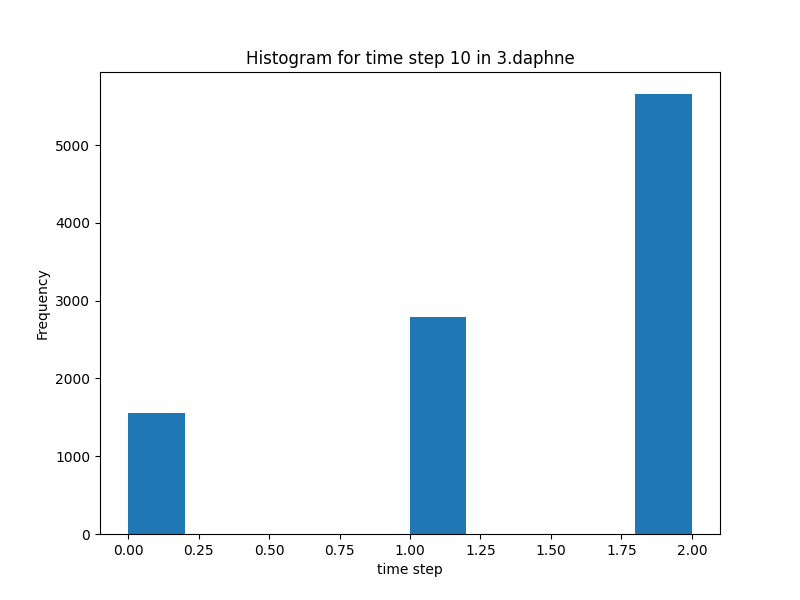
\includegraphics[width=0.24\textwidth]{../figs/4_daphne_10}%
        \label{fig:d}%
        }%
    \hfill%
    \subfloat[Samples from the prior for HMM step 11]{%
        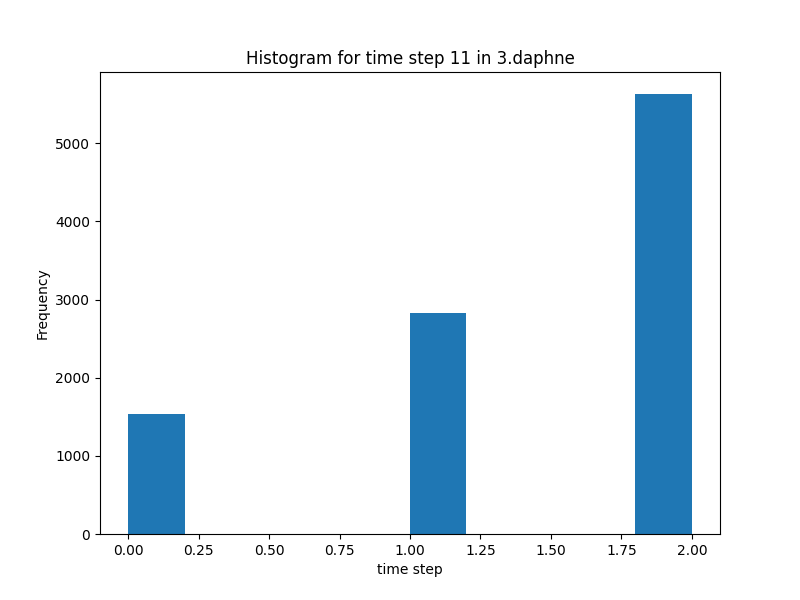
\includegraphics[width=0.24\textwidth]{../figs/4_daphne_11}%
        \label{fig:e}%
        }%
   \hfill%
   \subfloat[Samples from the prior for HMM step 12]{%
   	  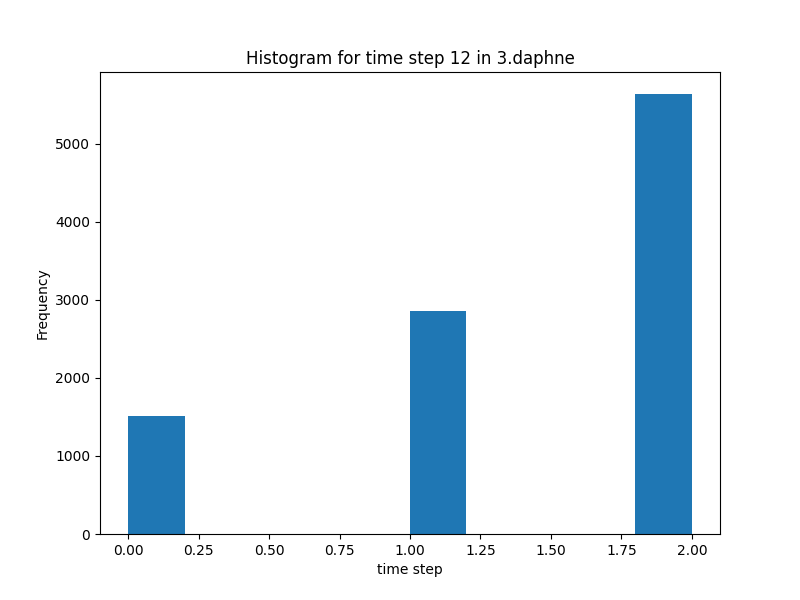
\includegraphics[width=0.24\textwidth]{../figs/4_daphne_12}%
   	  \label{fig:f}%
   	  }%
   	  
  \centering
   \subfloat[Samples from the prior for HMM step 13]{%
   	  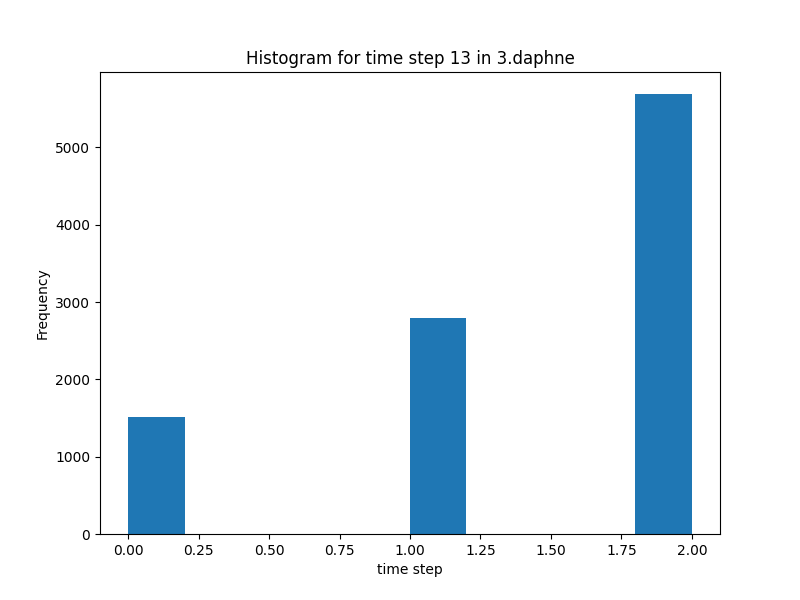
\includegraphics[width=0.24\textwidth]{../figs/4_daphne_13}%
   	  \label{fig:f}%
   	  }%
   \hfill%
   	  \subfloat[Samples from the prior for HMM step 14]{%
        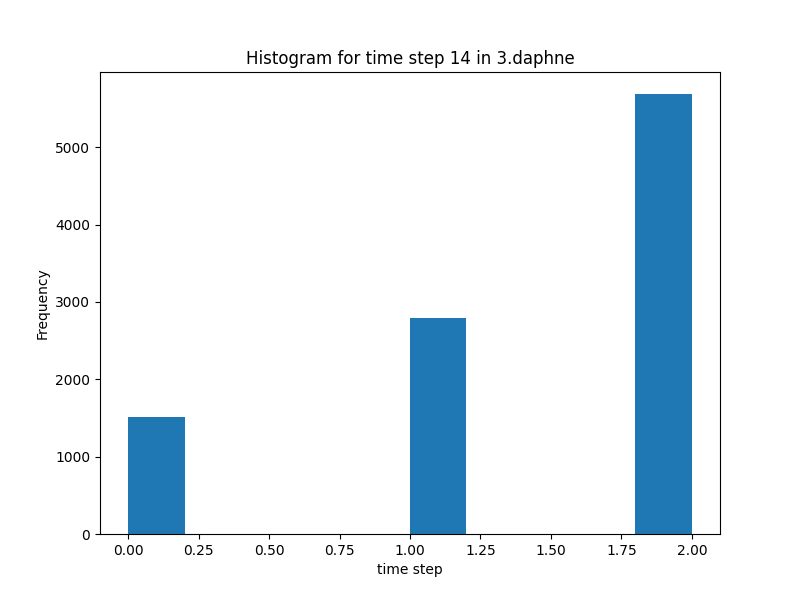
\includegraphics[width=0.24\textwidth]{../figs/4_daphne_14}%
        \label{fig:d}%
        }%
    \hfill%
    \subfloat[Samples from the prior for HMM step 15]{%
        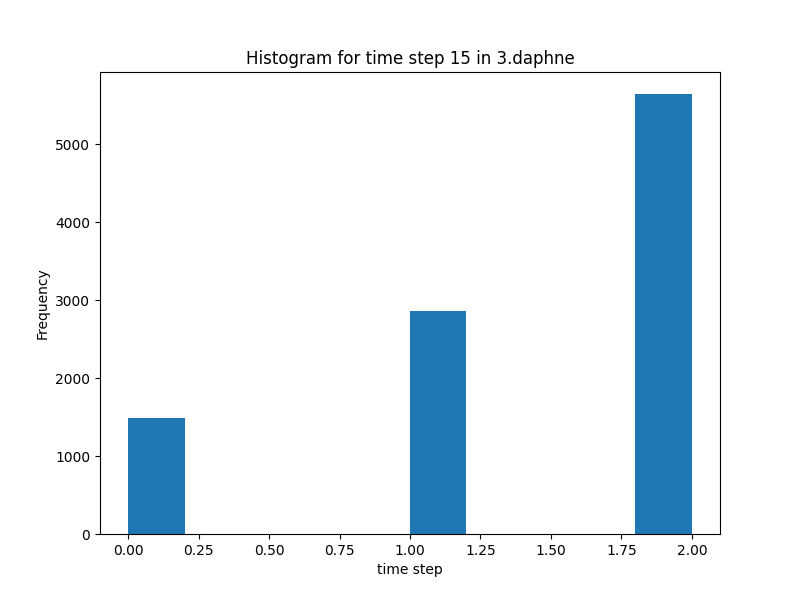
\includegraphics[width=0.24\textwidth]{../figs/4_daphne_15}%
        \label{fig:e}%
        }%
   \hfill%
   \subfloat[Samples from the prior for HMM step 16]{%
   	  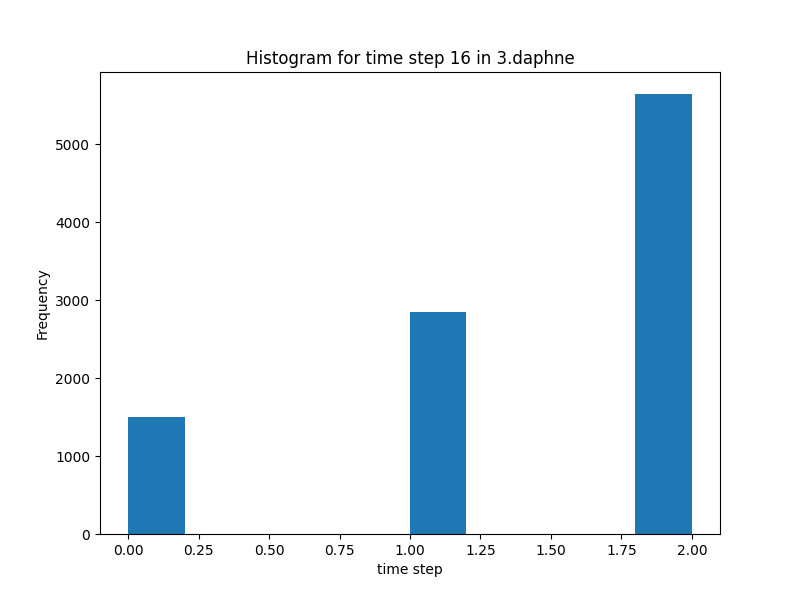
\includegraphics[width=0.24\textwidth]{../figs/4_daphne_16}%
   	  \label{fig:f}%
   	  }%
   \centering
   \subfloat[Samples from the prior for HMM step 17]{%
   	  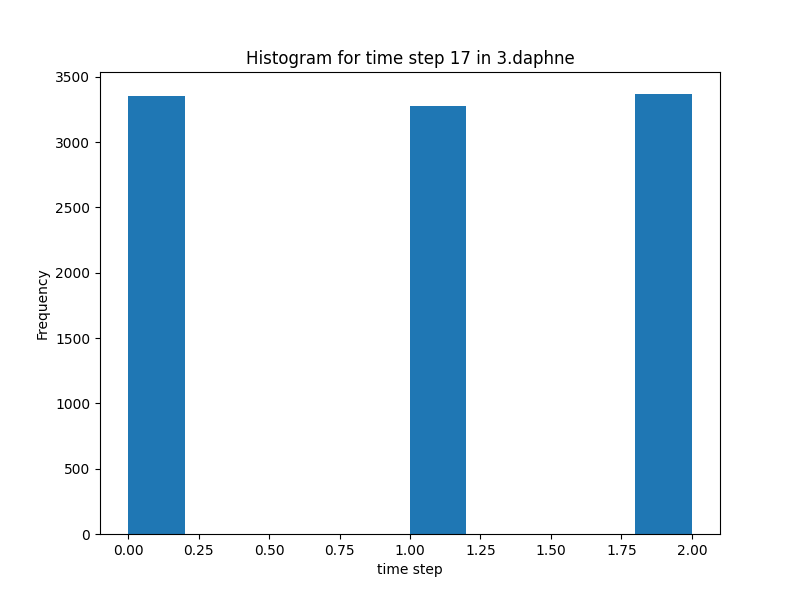
\includegraphics[width=0.24\textwidth]{../figs/4_daphne_17}%
   	  \label{fig:f}%
   	  }%
  
  \caption{Evaluation: Partial Histograms for 3.daphne}
 
\end{figure}

\end{enumerate}

\end{document}